\chapter{Results and discussion}
\label{chap:Results and discussion}

This chapter presents the experimental results obtained from the performance analysis that is delineated in \autoref{chap:Research methods}. For an impartial assessment of all models tested during training, a random 10\% holdout set of test triples was used. The holdout set is not seen by the models during training or validation. This strategy ensures fair evaluation of each model's generalization capabilities to new unseen data. To lay a solid framework for repeatability in future research experiments, throughout the analysis, a consistent set of training setup choices and hyperparameters was maintained, as detailed in \autoref{DEFAULT_PARAMS}.

\begin{table}
\caption{Default Training Setup Choices and Hyperparameters}
\label{DEFAULT_PARAMS}
\centering
\begin{tabular}{|c|c|c|c|c|c|}
\hline
\multirow[t]{2}{*}{\textbf{Parameter}} & \multicolumn{5}{c|}{\textbf{Value By Approach}} \bigstrut \\
\cline{2-6} 
& ComplEx & DistMult & RotatE & TransE & TransH \bigstrut \\
\hline 
Embedding Dim & 50 & 50 & 200 & 50 & 50 \\
\hline 
Num Epochs & \multicolumn{5}{c|}{500} \\
\hline 
Learning Rate & \multicolumn{5}{c|}{0.02} \\
\hline 
Num Negatives & \multicolumn{5}{c|}{1} \\
\hline
 % & \multicolumn{5}{c|}{} \\
% \hline
Optimizer & \multicolumn{5}{c|}{Adagrad} \\
\hline 
Inverse Relations & \multicolumn{5}{c|}{False} \\
\hline 
Loss Function & \multicolumn{5}{c|}{Margin Ranking Loss (Margin 1.0)} \\
\hline
\end{tabular}
\end{table}

\begin{figure}[!ht]
    \centering
    \begin{subfigure}[b]{1\textwidth}
        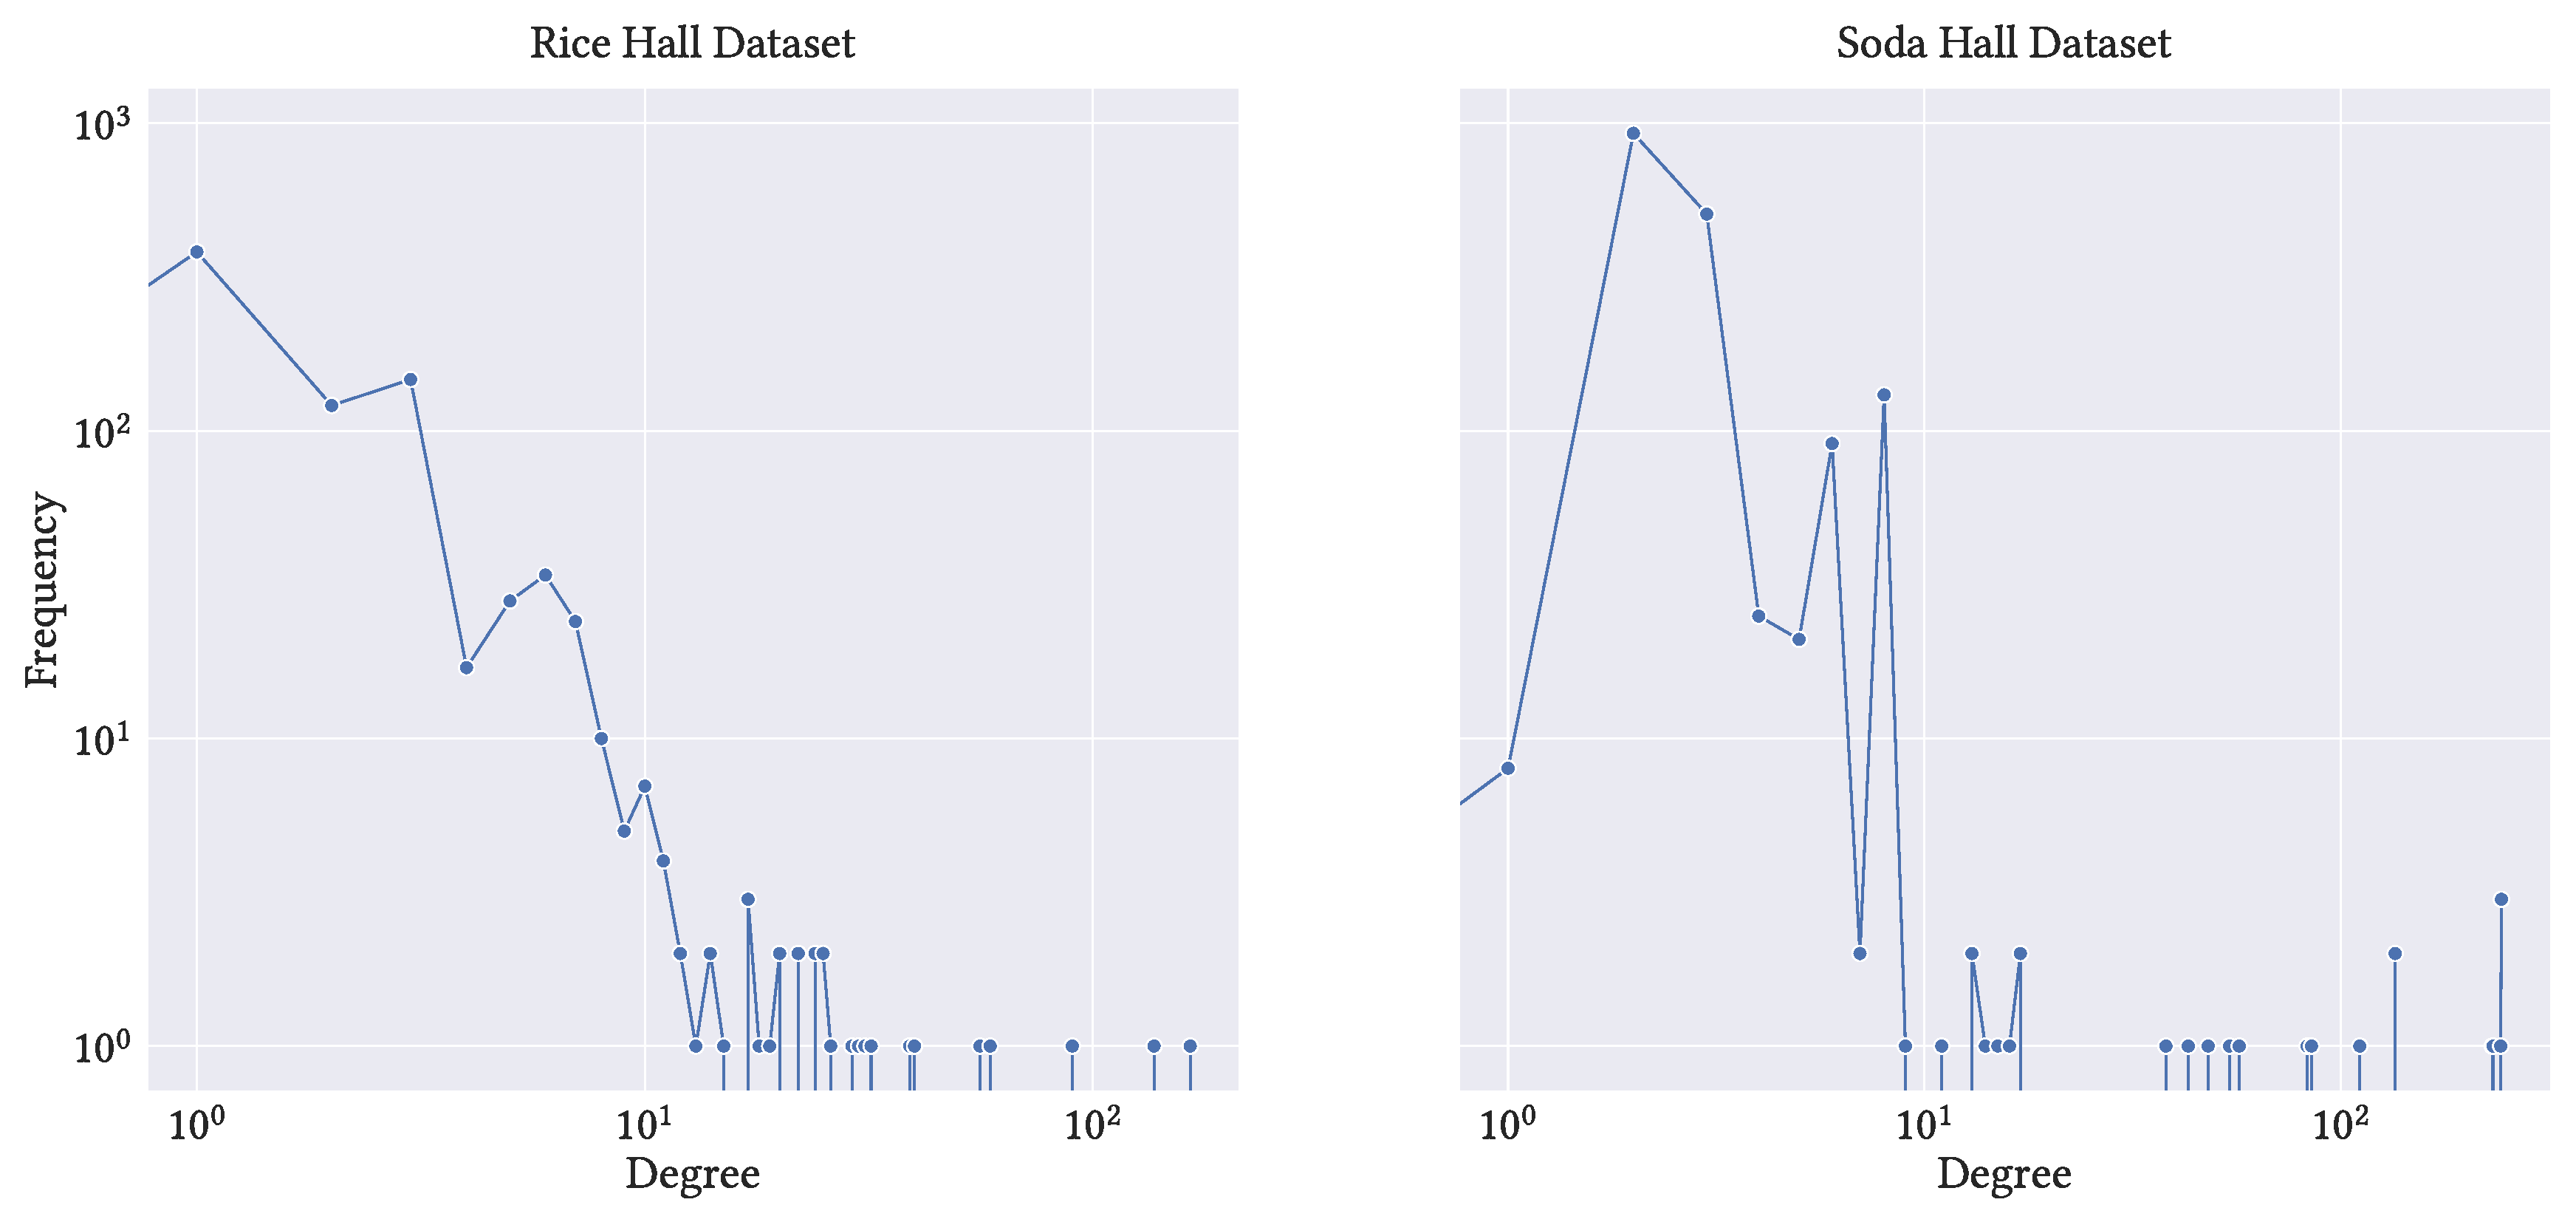
\includegraphics[width=\textwidth]{figures/Degree-distribution.eps}
        \caption{Degree distribution}
        \label{subfig:degree_distribution}
    \end{subfigure}
    % Spacing between subfigures. Adjust as needed.
    \vspace{1em}
    \begin{subfigure}[b]{1\textwidth}
        \includegraphics[width=\textwidth]{figures/kg-characteristics.eps}
        \caption{Relation cardinality types and relation patterns}
        \label{subfig:relation_cardinality_types_and_relation_patterns}
    \end{subfigure}
    \caption{Training dataset degree distributions, relation cardinality types and relation patterns }
    \label{fig:graph_characteristics}
\end{figure}

\section{A study on training setup choices}\label{sec: training setup choices}
The initial series of experiments aims to evaluate the influence of different categorical decisions related to the training configuration of \ac{KRL} models. In particular, this method varies the optimizer (selecting from a choice of Adam \citep{Kingma2014Adam:Optimization}, AdaGrad \citep{DuchiJohn2011AdaptiveOptimization} and \ac{SGD} \citep{Bottou1998OnlineApproximations}), training objective function (selecting from a choice of \ac{BCEL} \citep{Dettmers2017ConvolutionalEmbeddings}, \ac{SPL} \citep{Glorot2011DeepNetworks}, \ac{MRL} \citep{Bordes2013}, and the self-adversarial loss (NSSA) \citep{Sun2019RotatE:Space}), and finally considering the exclusion or inclusion of inverse relationships in the \ac{BIM-KG}s, a process that involves adding a copy of each triple during training but with an inverse relation.
A summary of the above categorical choices is presented in \autoref{tab:training_setup_choice_matrix}. 

\begin{table}
  \centering
  \caption{Training Setup Choice Matrix}
  \label{tab:training_setup_choice_matrix}
  \begin{tabular}{|c|c|c|c|}
    \hline
    \textbf{Model} & \textbf{Optimizer} & \textbf{Loss Function} & \textbf{Inverse Relationship} \bigstrut \\ \hline
    \multirow{18}{*}{All models} & \multirow{6}{*}{Adagrad} & \multirow{2}{*}{Binary Cross Entropy Loss (BCEL)} & False \\ \cline{4-4}
     &  &  & True \\ \cline{3-4}
     &  & \multirow{2}{*}{Softplus Loss (SPL)} & False \\ \cline{4-4}
     &  &  & True \\ \cline{3-4}
     &  & \multirow{2}{*}{Margin Ranking Loss (MRL)} & False \\ \cline{4-4}
     &  &  & True \\ \cline{2-4}
     & \multirow{6}{*}{Adam} & \multirow{2}{*}{Binary Cross Entropy Loss (BCEL) } & False \\ \cline{4-4}
     &  &  & True \\ \cline{3-4}
     &  & \multirow{2}{*}{Softplus Loss (SPL)} & False \\ \cline{4-4}
     &  &  & True \\ \cline{3-4}
     &  & \multirow{2}{*}{Margin Ranking (MRL)} & False \\ \cline{4-4}
     &  &  & True \\ \cline{2-4}
     & \multirow{6}{*}{SGD} & \multirow{2}{*}{Binary Cross Entropy Loss (BCEL)} & False \\ \cline{4-4}
     &  &  & True \\ \cline{3-4}
     &  & \multirow{2}{*}{Softplus Loss (SPL)} & False \\ \cline{4-4}
     &  &  & True \\ \cline{3-4}
     &  & \multirow{2}{*}{Margin Ranking Loss (MRL)} & False \\ \cline{4-4}
     &  &  & True \\ \hline
    % Repeat for other models like DistMult, RotatE, etc.
  \end{tabular}
\end{table}

\begin{figure}[!b]
    \centering
    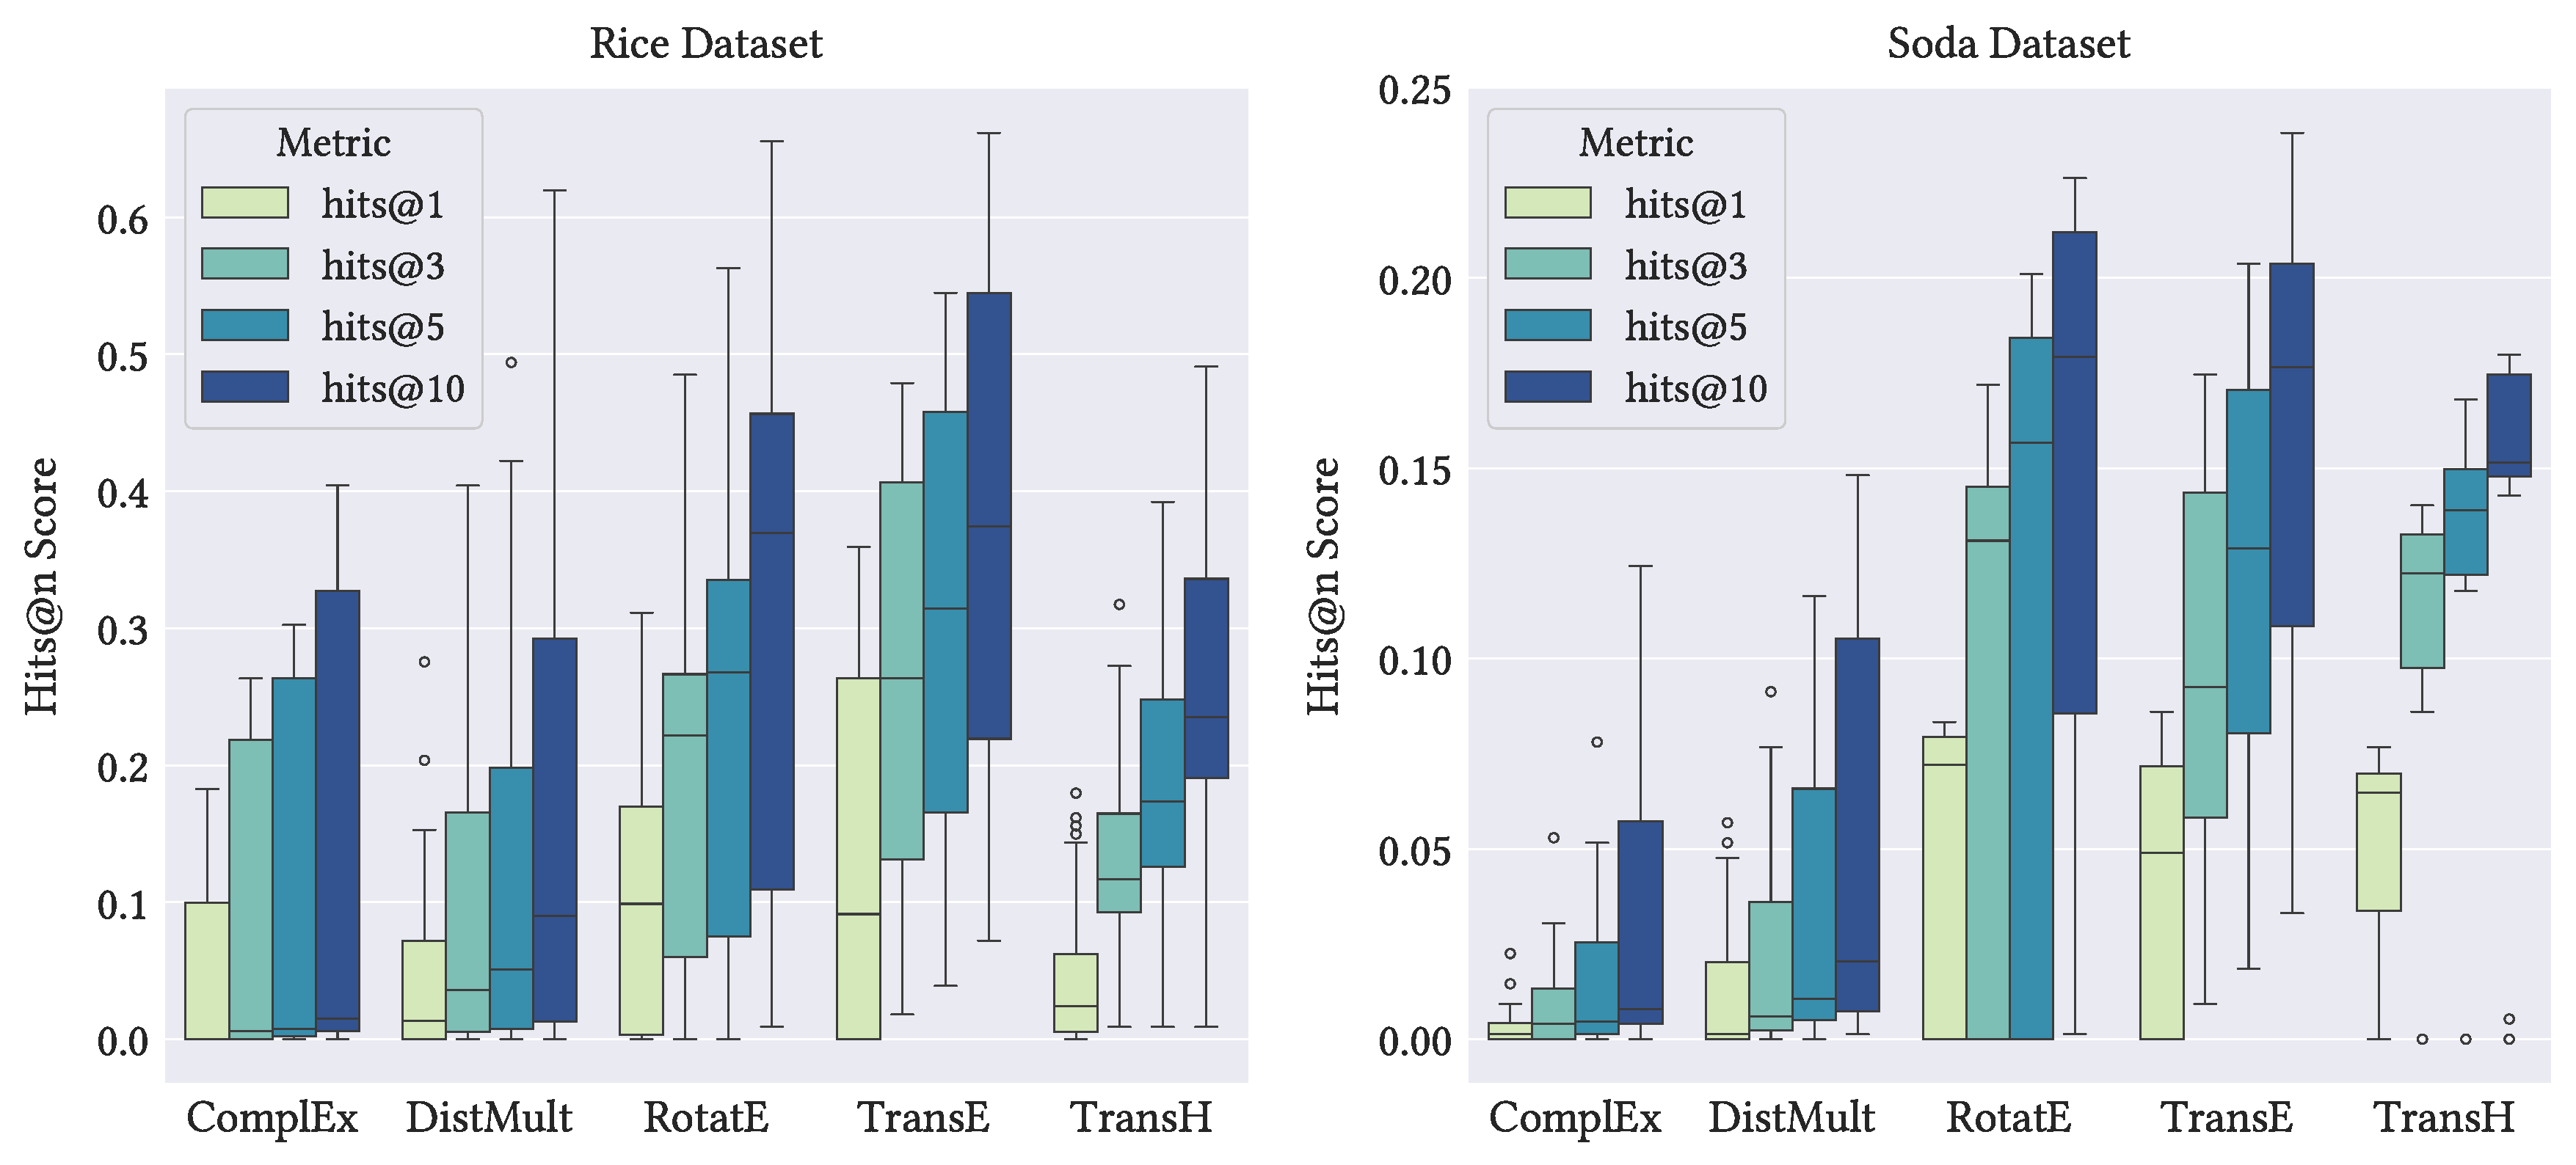
\includegraphics[width=1\textwidth]{figures/hits@10_across_all_models.eps}
    \caption{Distribution of Hits@$n$ (where $n \in \{1, 3, 5, 10\}$) scores across all categorial training setup choices.} \label{hits@10_across_all_models}
\end{figure}
\begin{figure}[!ht]
    \centering
    \begin{subfigure}[b]{\textwidth}
        \centering
        \includegraphics[width=1\textwidth]{figures/hits@10_across_all_models_and_optimizers.eps}
        \caption{Distribution of Hits@10 scores across all models and optimizers.}
        \label{subfig:hits@10_across_all_models_and_optimizers}
    \end{subfigure}
    
    \begin{subfigure}[b]{\textwidth}
        \centering
        \includegraphics[width=1\textwidth]{figures/hits@10_across_all_models_and_loss_functions.eps}
        \caption{Distribution of Hits@10 scores across all models and loss functions.}
        \label{subfig:hits@10_across_all_models_and_loss_functions}
    \end{subfigure}
    
    \begin{subfigure}[b]{\textwidth}
        \centering
        \includegraphics[width=1\textwidth]{figures/hits@10_across_all_models_with_inverse_relations_present_or_absent.eps}
        \caption{Distribution of Hits@10 scores across all models with inverse relations present or absent.}
        \label{subfig:hits@10_across_all_models_with_inverse_relations_present_or_absent}
    \end{subfigure}
    
    \caption{The effect of different training setup choices across all models and both datasets.}
    \label{fig: effect of different training setup choices across all models and both datasets}
\end{figure}

\Autoref{hits@10_across_all_models} depicts the Hits@10 scores distribution on the test set for different training setup options for all models and datasets. It offers detailed insight into how the models react to variations in the training setup. In the case of the Rice Hall dataset, all models show a comparable performance range, with TransE and RotatE standing out as the highest performers, whereas DistMult and ComplEx consistently show subpar performance no matter the training setup, a trend that can also be seen on the Soda Hall dataset, albeit happening more aggressively. DistMult inherently assumes symmetric relations due to its bilinear scoring function. However, many relationships in both datasets, such as \texttt{feeds} or \texttt{isPartOf}, are inherently directional (asymmetric). ComplEx attempts to address this by extending DistMult to complex numbers, allowing it to capture both symmetric and asymmetric relations. Despite this, the real challenge lies in the nuanced, hierarchical, and interdependent relationships typical of \acp{BIM-KG}, which ComplEx may not fully capture due to its inability to infer composition patterns. Composition patterns allow a building's multi-faceted relationships to be represented in knowledge graph embeddings. For example, the temperature in a room might be influenced by the operation of \ac{HVAC} systems, the number of inhabiting occupants, time of day, and even external weather conditions. Expressive capture of such patterns can enable an automation agent to predict the impact of adjusting the configurations of one system (like the \ac{HVAC} settings) on various related metrics (such as energy consumption or occupant comfort). Also, buildings often have a hierarchical structure: composed of floors, floors are composed of rooms, and rooms can contain various elements, sensors or actuators. Composition patterns in embeddings can reflect this hierarchy, allowing automation agents to aggregate or disaggregate information at different levels. For instance, understanding the aggregated energy use at the overall building level while also being able to drill down into specific floors or rooms. It is also important to note that \acp{BIM-KG} are often characterized by sparse data, with many potential but unobserved relationships between entities, which sparsity challenges the generalization capacity of these models. TransE and RotatE are less susceptible to overfitting in sparse environments because they embody lower complexity through their respective translational and geometric operations i.e., TransE needs a single vector to represent each relation as a translation in the embedding space, while RotatE requires a single complex number to represent each relation as a rotation. The lower number of parameters reduces the models' capacity to fit noise, a common pitfall in sparse datasets where the signal-to-noise ratio \footnote{Signal-to-noise ratio is defined as the ratio of meaningful input to meaningless or unwanted input} can be low. Perhaps the most striking observation is that RotatE generally demonstrates superior performance across both datasets, however, as seen in the Rice Hall dataset, older methods, such as TransE, can outperform it if given an optimized training setup. 

To further explore the effects of various training configurations, other distributions of model performance (Hits@10) for both datasets are presented in \autoref{subfig:hits@10_across_all_models_and_optimizers} through \autoref{subfig:hits@10_across_all_models_with_inverse_relations_present_or_absent}, revealing some intriguing patterns based on the different choices made. \Autoref{subfig:hits@10_across_all_models_and_optimizers} indicates that the setups that utilize the Adam optimizer consistently outperform those that use Adagrad and SGD. Adam's adaptive learning rate mechanism and momentum updates likely contribute to its ability to converge faster and escape local minima more effectively. Adagrad also adopts adaptive learning rates, performing smaller updates for parameters associated with frequently occurring features, and larger updates for parameters associated with infrequent features. Adam and Adagrad's adaptive learning rate mechanisms make them particularly well suited for tasks with sparse data where some features frequently occur while others remain rare. However, the monotonic decreasing learning rate of Adagrad can pose challenges in certain scenarios. As the Adagrad algorithm accumulates squared gradients over time, the learning rates for all parameters continuously decrease. While this ensures stable and well-scaled updates, it may also cause the algorithm to prematurely and excessively reduce the learning rate. The poor performance of \ac{SGD} indicates that its simplistic updating mechanism faces challenges in effectively exploring the complex parameter space of \ac{KRL} models. Also \ac{SGD} does not incorporate adaptive learning rates which means that it treats all parameters equally, applying the same update magnitude across the board. This uniform approach does not account for the importance of different features within the data. It is important to note that, due to the \textit{no-free-lunch}\footnote{There is no single optimizer to that will always do better than any other optimizer} theorem, there is no one-size-fits-all optimizer; in reality, an optimizer's efficiency is highly reliant on the training setup and unique characteristics of the underlying dataset. This is evident in \autoref{subfig:hits@10_across_all_models_and_optimizers} (Soda Hall dataset), where for ComplEx, Adagrad performs worse than \ac{SGD}.

Looking at \autoref{subfig:hits@10_across_all_models_and_loss_functions} reveals similar performance for the \ac{BCEL} and the \ac{SPL} across both datasets. This is because \ac{SPL} is equivalent to \ac{BCEL} though numerically more stable. Even though \citep{Ali2020BringingFramework} claims that \ac{BCEL} is not well-suited for translational distance models, it exhibits competitive performance for TransE on the Soda Hall dataset and even surpasses the numerically more stable \ac{SPL}. These peculiarities highlight that identifying appropriate training configurations can produce results that deviate from what was previously known. Experimental evidence from the biological domain has shown that adding inverse relationships to the training knowledge graph performs worse than not including them; however, the results herein are contrasting as shown in \autoref{subfig:hits@10_across_all_models_with_inverse_relations_present_or_absent} where adding inverse relationships to the dataset configurations for ComplEx and RotatE yields better performance. In contrast, the same configuration leads to poor performance for TransH and DistMult for when trained on the Soda Hall Dataset. However, when trained on the Rice Hall dataset, Distmult and TransE perform similarly on average. Overall, \autoref{fig: effect of different training setup choices across all models and both datasets} has revealed how combinatorial the problem of configuring the training setup is. Another interesting observation is that improving training setups has proven to enhance performance more significantly than improving model architectures for instance, the older TransE model has been observed to outperform the newer RotatE model if it is configured suboptimally as is the case in \autoref{hits@10_across_all_models}. In \autoref{subfig:hpo_summary} showing the distribution of Hits@10 scores across all 100 trials using \ac{TPE} method, it is notable that all models are sensitive to the hyper-parameters which means that the best-performing model could easily be outperformed if not carefully tuned. 

\section{A study on \ac{HPO} choices}\label{sec: training setup choices}

\begin{figure}[!ht]
    \centering
    \begin{subfigure}[b]{\textwidth}
        \centering
        \includegraphics[width=1\textwidth]{figures/hpo_total_runtime.eps}
        \caption{Total \ac{HPO} runtimes for all models}
        \label{subfig:hpo_total_runtime}
    \end{subfigure}
    
    \begin{subfigure}[b]{\textwidth}
        \centering
        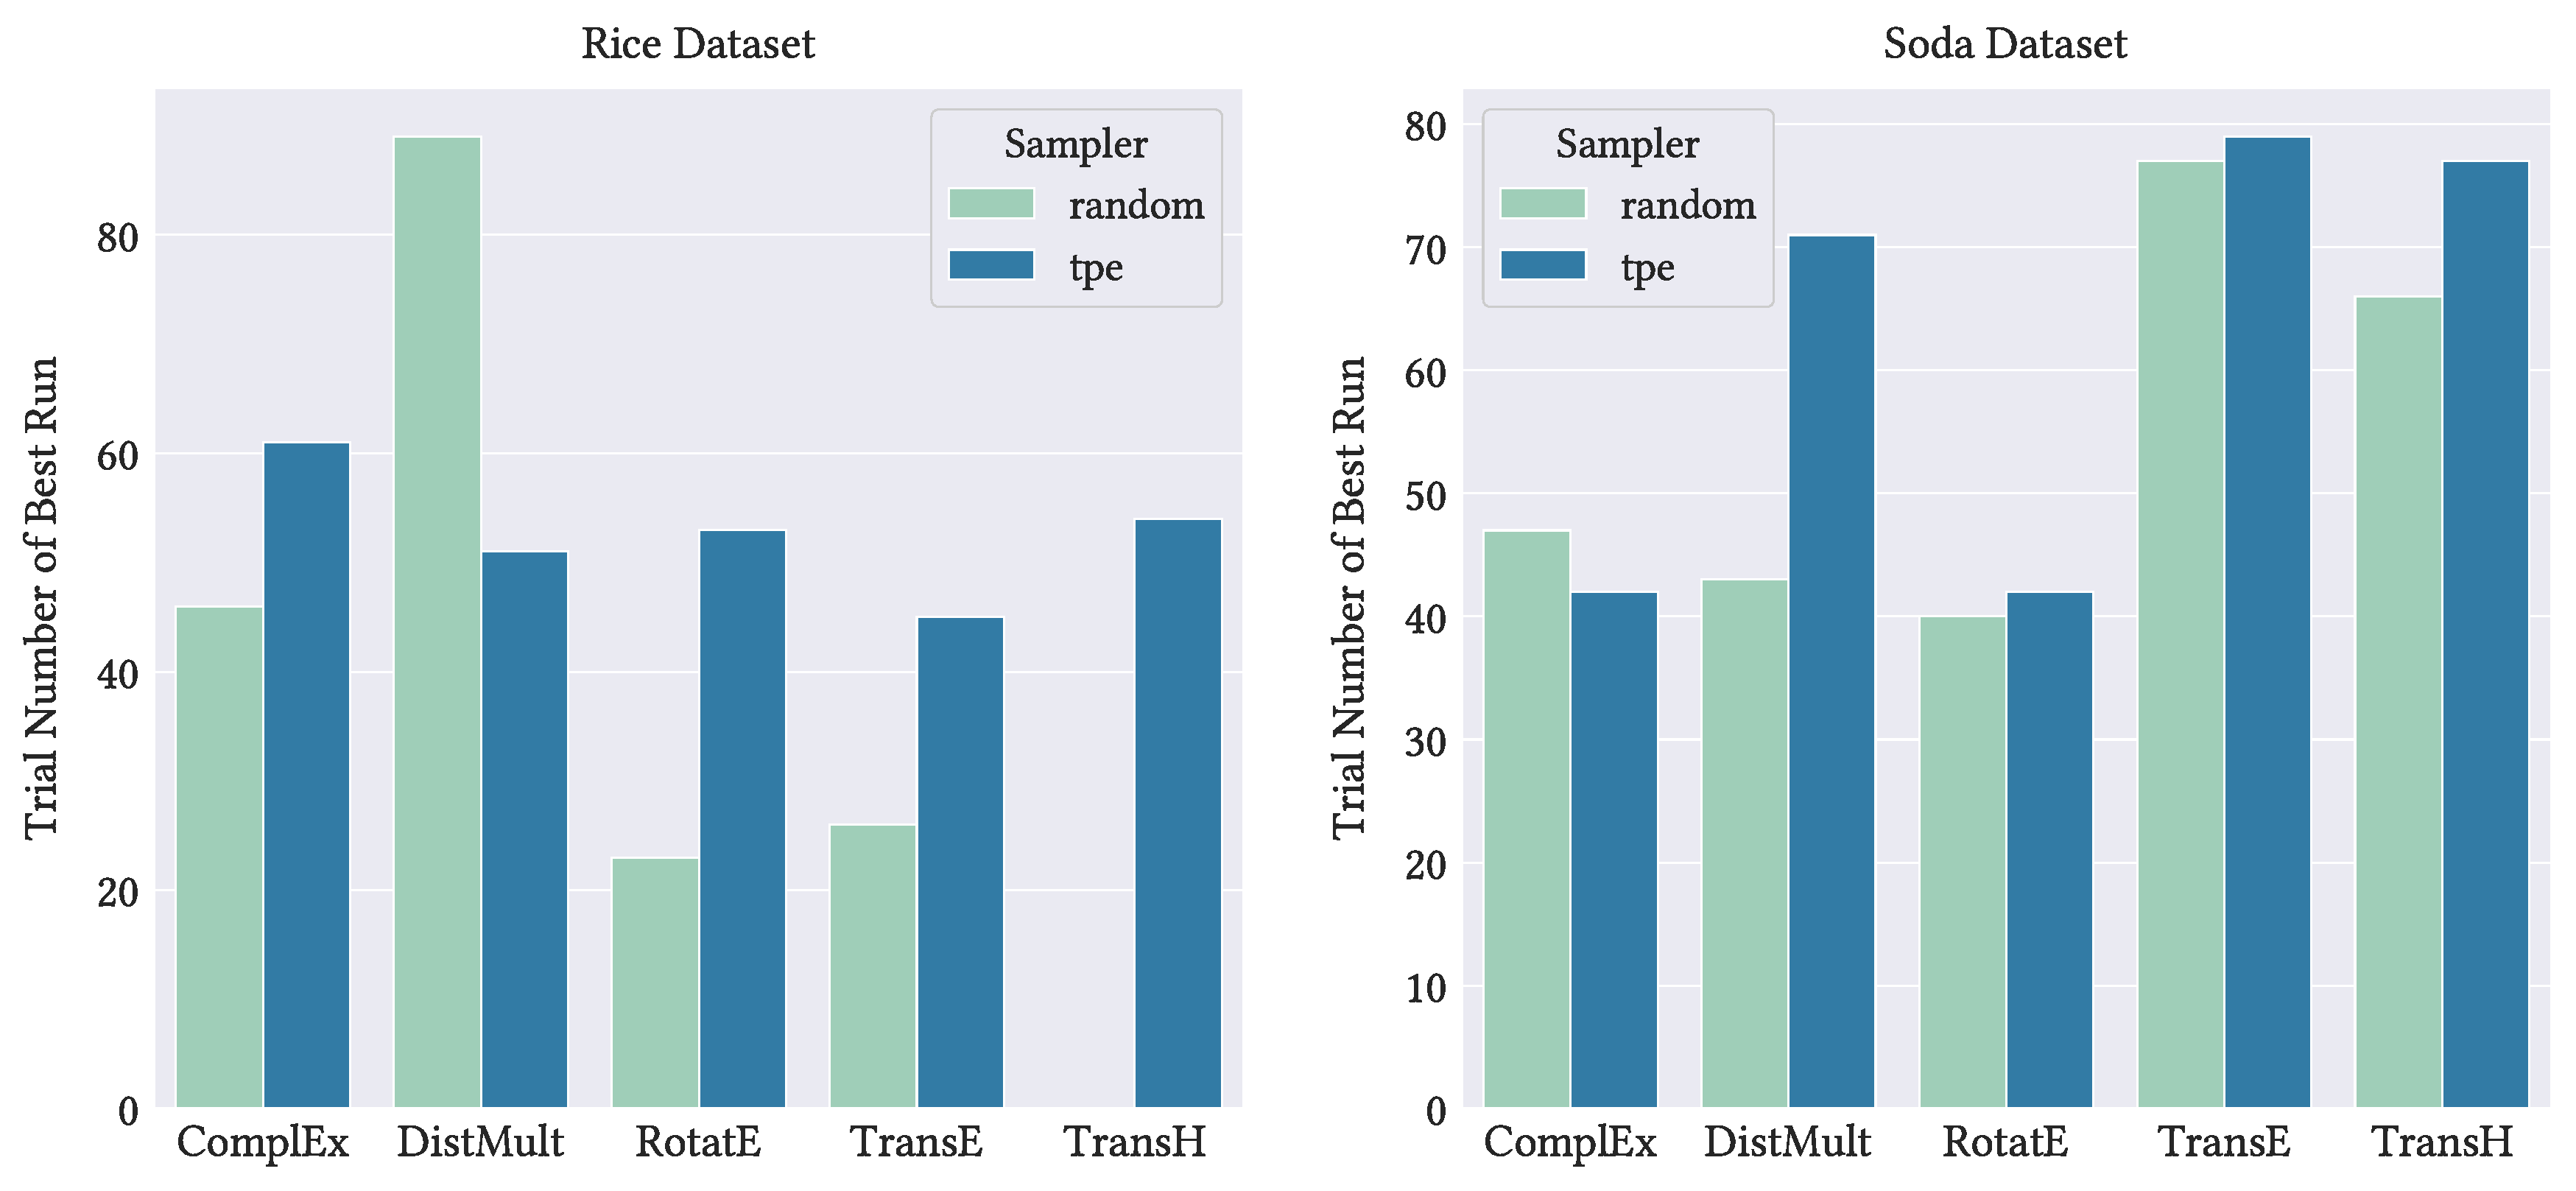
\includegraphics[width=1\textwidth]{figures/hpo_best_trial_number.eps}
        \caption{Best \ac{HPO} trial number for all models}
        \label{subfig:hpo_best_trial_number}
    \end{subfigure}
    
    \caption{The effect of 2 different \ac{HPO} strategies across all models and both datasets (Part 1).}
    \label{fig:effect_of_2_different_HPO_strategies_part1}
\end{figure}

\begin{figure}[!ht]
    \centering
    \begin{subfigure}[b]{\textwidth}
        \centering
        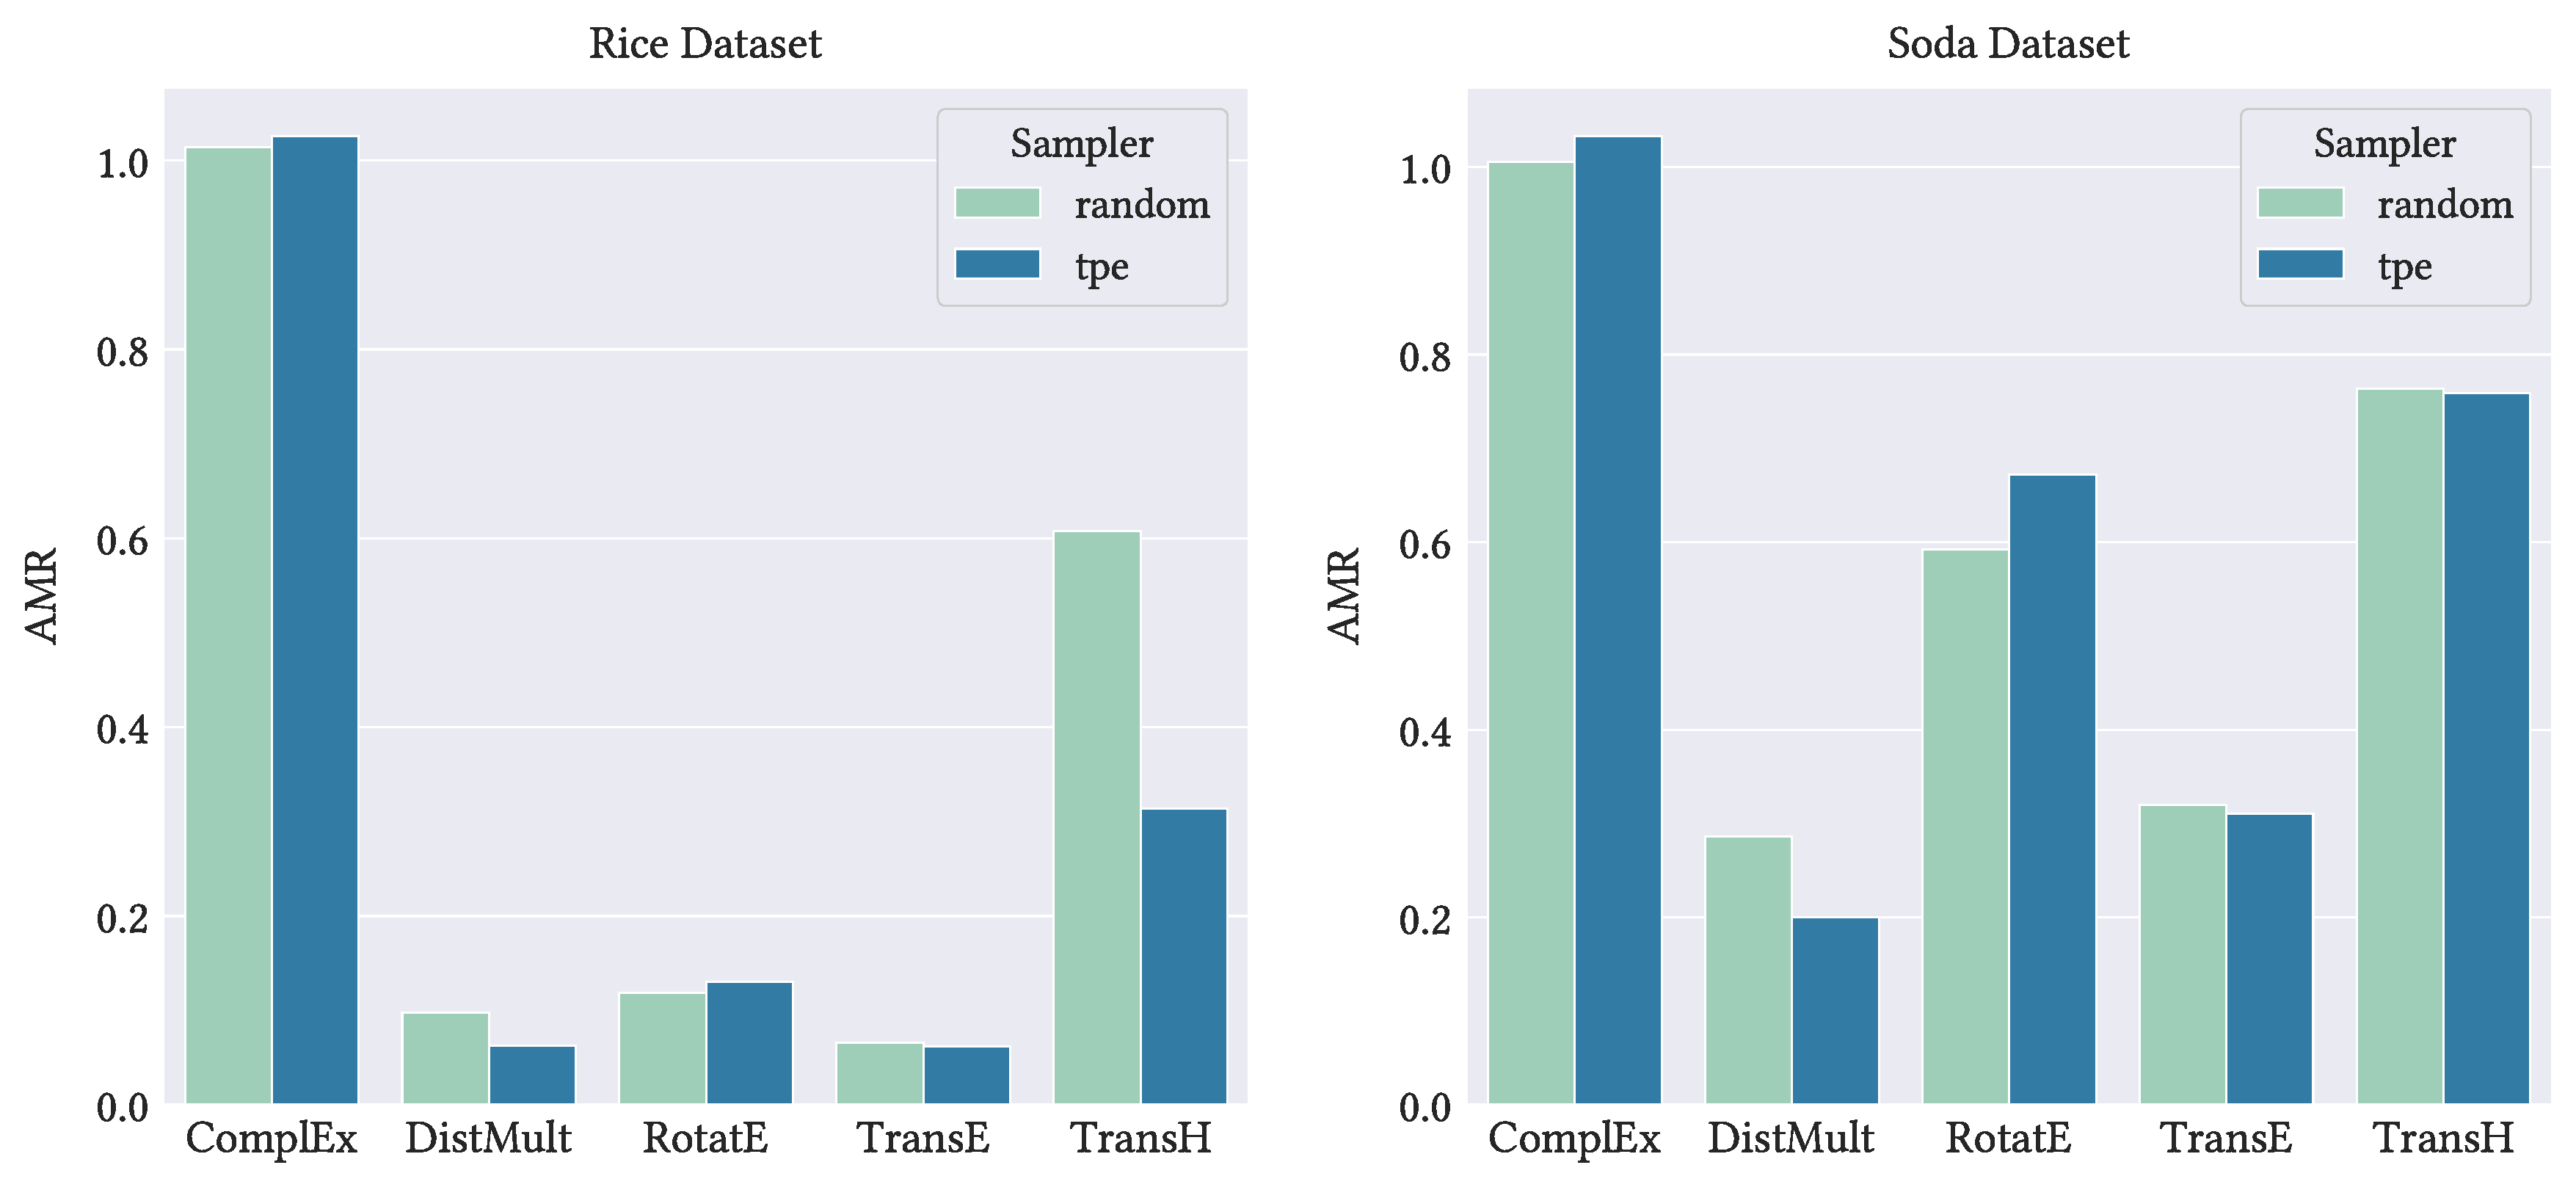
\includegraphics[width=1\textwidth]{figures/hpo_best_trial_AMR.eps}
        \caption{Best \ac{HPO} trial \ac{AMR}}
        \label{subfig:hpo_best_trial_AMR}
    \end{subfigure}
    
    \begin{subfigure}[b]{\textwidth}
        \centering
        \includegraphics[width=1\textwidth]{figures/hpo_best_trial_hits@10.eps}
        \caption{Best \ac{HPO} trial Hits@10}
        \label{subfig:hpo_best_trial_hits@10}
    \end{subfigure}
    
    \begin{subfigure}[b]{\textwidth}
        \centering
        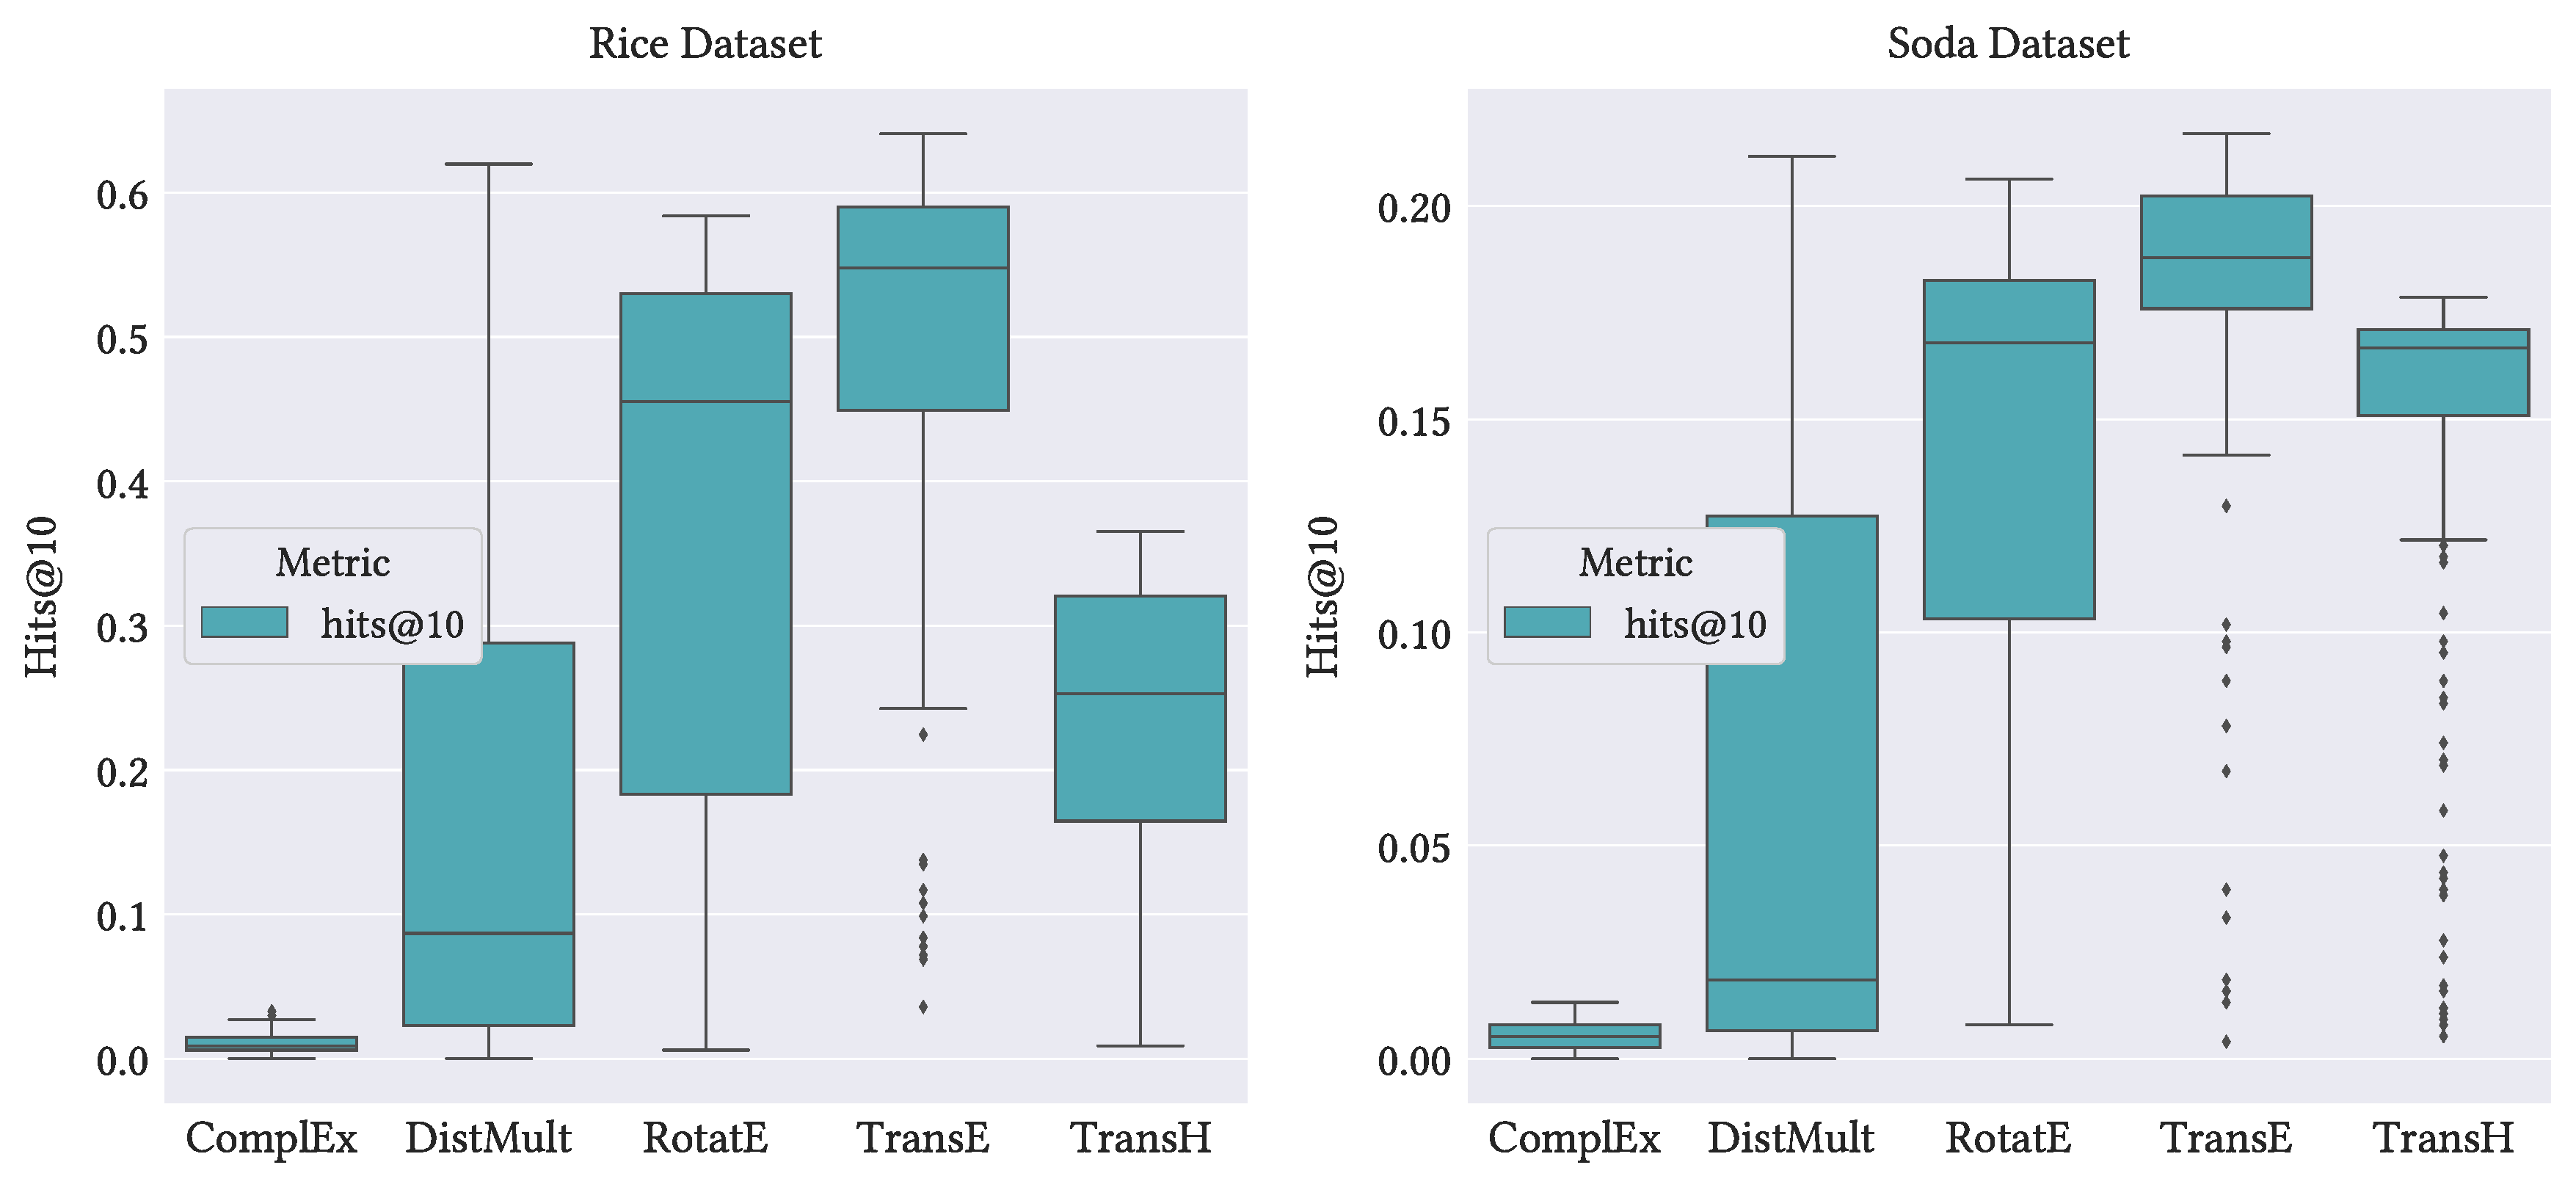
\includegraphics[width=1\textwidth]{figures/hpo_summary_overall_hits@10.eps}
        \caption{Distribution of Hits@10 Scores Across all HPO runs of all models}
        \label{subfig:hpo_summary}
    \end{subfigure}
    
    \caption{The effect of 2 different \ac{HPO} strategies across all models and both datasets (Part 2).}
    \label{fig:effect_of_2_different_HPO_strategies_part2}
\end{figure}

\begin{table}[t]
    \centering
    \begin{tabular}{ll}
    \hline \hline \textbf{Parameter} & \textbf{Value range} \bigstrut \\
    \hline Embedding Dim & {$[16 \ldots 512,16]$} \bigstrut \\
    Num Epochs & {$[10 \ldots 50,10]$} \bigstrut \\
    Learning Rate & {$[0.001 \ldots 0.1, \log ]$} \bigstrut \\
    Num Negatives & {$[1 \ldots 100,10]$} \bigstrut \\
    \hline
    \end{tabular}
    \caption{Range of search for \ac{HPO} values in the form of minimum, maximum and step.}
    \label{tab:hpo_search_range}
\end{table}

\noindent Even with a robust training configuration, the choice of hyperparameters can significantly affect the model performance. In this study's experiments, two \ac{HPO} search strategies are employed i.e., Bayesian \ac{TPE} \citep{Bergstra2011AlgorithmsOptimization} and random search \citep{Bergstra2012RandomOptimization}. In the Bayesian \ac{TPE}, a posterior distribution of the objective function is modelled and used to predict the performance of different hyperparameter configurations based on historical evaluations while random search selects hyperparameter configurations uniformly at random from a predefined range. For each strategy, 100 experiments are conducted without time constraints, using a fixed model seed, training setup (see \autoref{DEFAULT_PARAMS}), and hyperparameter optimization search ranges (see \autoref{tab:hpo_search_range}). The hyperparameters were evaluated using the AMR metric for both \ac{HPO} search strategies on a 10\% holdout set of triples that is randomly selected but fixed across all trials. Observing \autoref{subfig:hpo_total_runtime}, \ac{TPE} trials took a shorter time than random search on average. Even though \ac{TPE}'s parameter tuning strategies can increase runtime, it managed to achieve shorter trial runs than random search. \Autoref{subfig:hpo_best_trial_number} shows that on average, \ac{TPE} achieves its best performance closer to the maximum number of trials (100). Again this is likely due to the fact that \ac{TPE} can tune parameters that can increase run time significantly. In \autoref{subfig:hpo_best_trial_AMR} and \autoref{subfig:hpo_best_trial_hits@10}, it is interesting to see how close the performance of \ac{TPE} is to random search, with \ac{TPE} yielding only slightly better-performing models. While often considered more naive, random search can occasionally outperform sophisticated methods by randomly finding optimal parameters, potentially uncovering high-performing configurations that systematic searches may miss. Close observation of \autoref{subfig:hpo_best_trial_AMR} and \autoref{subfig:hpo_best_trial_hits@10}, shows a negative correlation between \ac{AMR} and Hits@10 which is nice to see as the \ac{HPO} was solely focused on optimising for \ac{AMR}.

\section{\acf{KRL-based BCF}}
\label{KRL-based BCF}
Because \ac{KRL} is an infant technique in the \ac{AEC/FM} field, formulating a reproducibility framework is deemed relevant and the main objective of this thesis. It is a two-fold process;
\begin{enumerate}
    \item 
    Summarizing the technical aspects and key considerations for building, evaluating and validating \acp{BIM-KG} for downstream \ac{KRL} pipelines.

    \begin{figure}[h]
    \centering
    \includegraphics[width=1\textwidth]{figures/lbd_for_krl.pdf}
    \caption{Summarized framework for building, evaluating and validating \acp{BIM-KG} for downstream \ac{KRL} pipelines}\label{SSN_OPM_SEAS}
\end{figure}

    \item 
    Using the deductions from the performance analysis experiments to define the prerequisites for integrating \ac{KRL} with \acp{BIM-KG} in a domain-independent framework.   
\end{enumerate}
\begin{figure}[!t]
        \centering
        \includegraphics[width=1\textwidth]{figures/LBD-KRL Framework.pdf}
        \caption{KRL-based BCF}\label{KRL-based BCF Chart}
    \end{figure}

\section{Framework Applicability / Implementation Setup}
This section summarizes a high-level framework implementation setup consisting of \ac{IoT} devices (see \autoref{DHT22 circuit}), and a prototype program of the framework \ac{API} (see \autoref{Framework implementation}). The \ac{API} consists of a server-side module and a client-side module. The server-side module can communicate with \ac{KRL} configurators, external services such as \ac{BIM-KG} databases, sensor data stores, and \ac{MQTT} brokers. The client-side module consists of a \ac{GUI} with a \ac{COBie} handler service that facilitates the curation of \acp{BIM-KG} from \ac{COBie} files and an interrogation service that facilitates declarative interrogation of the server-side module using \ac{SPARQL} and \ac{GraphQL}. This prototype demonstrates a use case where the resultant \ac{KRL} embeddings are used to enhance the accuracy and reliability of \acp{LLM} with building information sources fetched from external sources such as Microsoft Dynamics 365 via GraphQL and REST \ac{API}s.
\begin{figure}[h]
        \centering
        \includegraphics[width=1\textwidth]{figures/DHT22 Circuit.pdf}
        \caption{DHT22 Setup with ESP32 Micro controller}\label{DHT22 circuit}
\end{figure}
\begin{figure}[h]
    \centering
    \includegraphics[width=1\textwidth]{figures/Implementation.pdf}
    \caption{Framework Implementation Prototype Setup}\label{Framework implementation}
\end{figure}
    





